% Options for packages loaded elsewhere
% Options for packages loaded elsewhere
\PassOptionsToPackage{unicode}{hyperref}
\PassOptionsToPackage{hyphens}{url}
\PassOptionsToPackage{dvipsnames,svgnames,x11names}{xcolor}
%
\documentclass[
  letterpaper,
  DIV=11,
  numbers=noendperiod]{scrartcl}
\usepackage{xcolor}
\usepackage{amsmath,amssymb}
\setcounter{secnumdepth}{5}
\usepackage{iftex}
\ifPDFTeX
  \usepackage[T1]{fontenc}
  \usepackage[utf8]{inputenc}
  \usepackage{textcomp} % provide euro and other symbols
\else % if luatex or xetex
  \usepackage{unicode-math} % this also loads fontspec
  \defaultfontfeatures{Scale=MatchLowercase}
  \defaultfontfeatures[\rmfamily]{Ligatures=TeX,Scale=1}
\fi
\usepackage{lmodern}
\ifPDFTeX\else
  % xetex/luatex font selection
\fi
% Use upquote if available, for straight quotes in verbatim environments
\IfFileExists{upquote.sty}{\usepackage{upquote}}{}
\IfFileExists{microtype.sty}{% use microtype if available
  \usepackage[]{microtype}
  \UseMicrotypeSet[protrusion]{basicmath} % disable protrusion for tt fonts
}{}
\makeatletter
\@ifundefined{KOMAClassName}{% if non-KOMA class
  \IfFileExists{parskip.sty}{%
    \usepackage{parskip}
  }{% else
    \setlength{\parindent}{0pt}
    \setlength{\parskip}{6pt plus 2pt minus 1pt}}
}{% if KOMA class
  \KOMAoptions{parskip=half}}
\makeatother
% Make \paragraph and \subparagraph free-standing
\makeatletter
\ifx\paragraph\undefined\else
  \let\oldparagraph\paragraph
  \renewcommand{\paragraph}{
    \@ifstar
      \xxxParagraphStar
      \xxxParagraphNoStar
  }
  \newcommand{\xxxParagraphStar}[1]{\oldparagraph*{#1}\mbox{}}
  \newcommand{\xxxParagraphNoStar}[1]{\oldparagraph{#1}\mbox{}}
\fi
\ifx\subparagraph\undefined\else
  \let\oldsubparagraph\subparagraph
  \renewcommand{\subparagraph}{
    \@ifstar
      \xxxSubParagraphStar
      \xxxSubParagraphNoStar
  }
  \newcommand{\xxxSubParagraphStar}[1]{\oldsubparagraph*{#1}\mbox{}}
  \newcommand{\xxxSubParagraphNoStar}[1]{\oldsubparagraph{#1}\mbox{}}
\fi
\makeatother


\usepackage{longtable,booktabs,array}
\usepackage{calc} % for calculating minipage widths
% Correct order of tables after \paragraph or \subparagraph
\usepackage{etoolbox}
\makeatletter
\patchcmd\longtable{\par}{\if@noskipsec\mbox{}\fi\par}{}{}
\makeatother
% Allow footnotes in longtable head/foot
\IfFileExists{footnotehyper.sty}{\usepackage{footnotehyper}}{\usepackage{footnote}}
\makesavenoteenv{longtable}
\usepackage{graphicx}
\makeatletter
\newsavebox\pandoc@box
\newcommand*\pandocbounded[1]{% scales image to fit in text height/width
  \sbox\pandoc@box{#1}%
  \Gscale@div\@tempa{\textheight}{\dimexpr\ht\pandoc@box+\dp\pandoc@box\relax}%
  \Gscale@div\@tempb{\linewidth}{\wd\pandoc@box}%
  \ifdim\@tempb\p@<\@tempa\p@\let\@tempa\@tempb\fi% select the smaller of both
  \ifdim\@tempa\p@<\p@\scalebox{\@tempa}{\usebox\pandoc@box}%
  \else\usebox{\pandoc@box}%
  \fi%
}
% Set default figure placement to htbp
\def\fps@figure{htbp}
\makeatother





\setlength{\emergencystretch}{3em} % prevent overfull lines

\providecommand{\tightlist}{%
  \setlength{\itemsep}{0pt}\setlength{\parskip}{0pt}}



 


\KOMAoption{captions}{tableheading}
\makeatletter
\@ifpackageloaded{caption}{}{\usepackage{caption}}
\AtBeginDocument{%
\ifdefined\contentsname
  \renewcommand*\contentsname{Table of contents}
\else
  \newcommand\contentsname{Table of contents}
\fi
\ifdefined\listfigurename
  \renewcommand*\listfigurename{List of Figures}
\else
  \newcommand\listfigurename{List of Figures}
\fi
\ifdefined\listtablename
  \renewcommand*\listtablename{List of Tables}
\else
  \newcommand\listtablename{List of Tables}
\fi
\ifdefined\figurename
  \renewcommand*\figurename{Figure}
\else
  \newcommand\figurename{Figure}
\fi
\ifdefined\tablename
  \renewcommand*\tablename{Table}
\else
  \newcommand\tablename{Table}
\fi
}
\@ifpackageloaded{float}{}{\usepackage{float}}
\floatstyle{ruled}
\@ifundefined{c@chapter}{\newfloat{codelisting}{h}{lop}}{\newfloat{codelisting}{h}{lop}[chapter]}
\floatname{codelisting}{Listing}
\newcommand*\listoflistings{\listof{codelisting}{List of Listings}}
\makeatother
\makeatletter
\makeatother
\makeatletter
\@ifpackageloaded{caption}{}{\usepackage{caption}}
\@ifpackageloaded{subcaption}{}{\usepackage{subcaption}}
\makeatother
\usepackage{bookmark}
\IfFileExists{xurl.sty}{\usepackage{xurl}}{} % add URL line breaks if available
\urlstyle{same}
\hypersetup{
  pdftitle={ITIL 4},
  pdfauthor={Joao Luiz D'Andrea},
  colorlinks=true,
  linkcolor={blue},
  filecolor={Maroon},
  citecolor={Blue},
  urlcolor={Blue},
  pdfcreator={LaTeX via pandoc}}


\title{ITIL 4}
\usepackage{etoolbox}
\makeatletter
\providecommand{\subtitle}[1]{% add subtitle to \maketitle
  \apptocmd{\@title}{\par {\large #1 \par}}{}{}
}
\makeatother
\subtitle{Service Management and Value Co-Creation Framework}
\author{Joao Luiz D'Andrea}
\date{}
\begin{document}
\maketitle

\renewcommand*\contentsname{Table of contents}
{
\hypersetup{linkcolor=}
\setcounter{tocdepth}{3}
\tableofcontents
}

\section{Overview}\label{overview}

\subsection{What is ITIL 4}\label{what-is-itil-4}

ITIL 4 is a service management framework used to design, deliver,
operate, and continually improve services. It moves beyond a narrow
process view and frames service management as a system for co-creating
value with customers, users, suppliers, and internal stakeholders.

ITIL 4 is centred on the \textbf{Service Value System (SVS)}, the
\textbf{Service Value Chain}, the \textbf{Four Dimensions of Service
Management}, and a set of practices that help organisations translate
strategy into reliable and improving service outcomes.

It is useful not only in traditional IT operations but also in digital
product management, platform teams, cloud operations, enterprise support
functions, and cross-functional service organisations.

\subsection{Purpose}\label{purpose}

The purpose of ITIL 4 is to help organisations:

\begin{itemize}
\tightlist
\item
  align services with business outcomes and customer value;
\item
  establish a common operating model for design, transition, support,
  and improvement;
\item
  improve reliability, responsiveness, and service experience;
\item
  create consistent governance and accountability across service teams;
\item
  support digital transformation through adaptable practices rather than
  rigid process bureaucracy; and
\item
  embed continual improvement into daily operations and strategic
  change.
\end{itemize}

\subsection{When to Use It}\label{when-to-use-it}

ITIL 4 is especially useful when an organisation needs a coherent
service management model across operations, support, delivery, and
supplier ecosystems. Common situations include:

\begin{itemize}
\tightlist
\item
  establishing or improving IT service management;
\item
  modernising service desk, incident, problem, and change practices;
\item
  introducing service ownership and service catalogue management;
\item
  improving end-to-end service design and transition controls;
\item
  integrating Agile, DevOps, product, and operations ways of working;
\item
  improving customer experience and service-level performance; and
\item
  strengthening governance over outsourced or multi-supplier
  environments.
\end{itemize}

\subsection{Target Audience}\label{target-audience}

\begin{itemize}
\tightlist
\item
  CIO
\item
  Head of IT Service Management
\item
  Service Management Office / SMO
\item
  Service Owners
\item
  Operations Managers
\item
  Service Desk Leaders
\item
  Change, Incident, and Problem Managers
\item
  Supplier Managers
\item
  Enterprise Architects
\item
  PMO / Transformation Office
\item
  Risk, compliance, and audit teams
\item
  Digital product and platform leaders
\end{itemize}

\subsection{ITIL 4 Service Value
System}\label{itil-4-service-value-system}

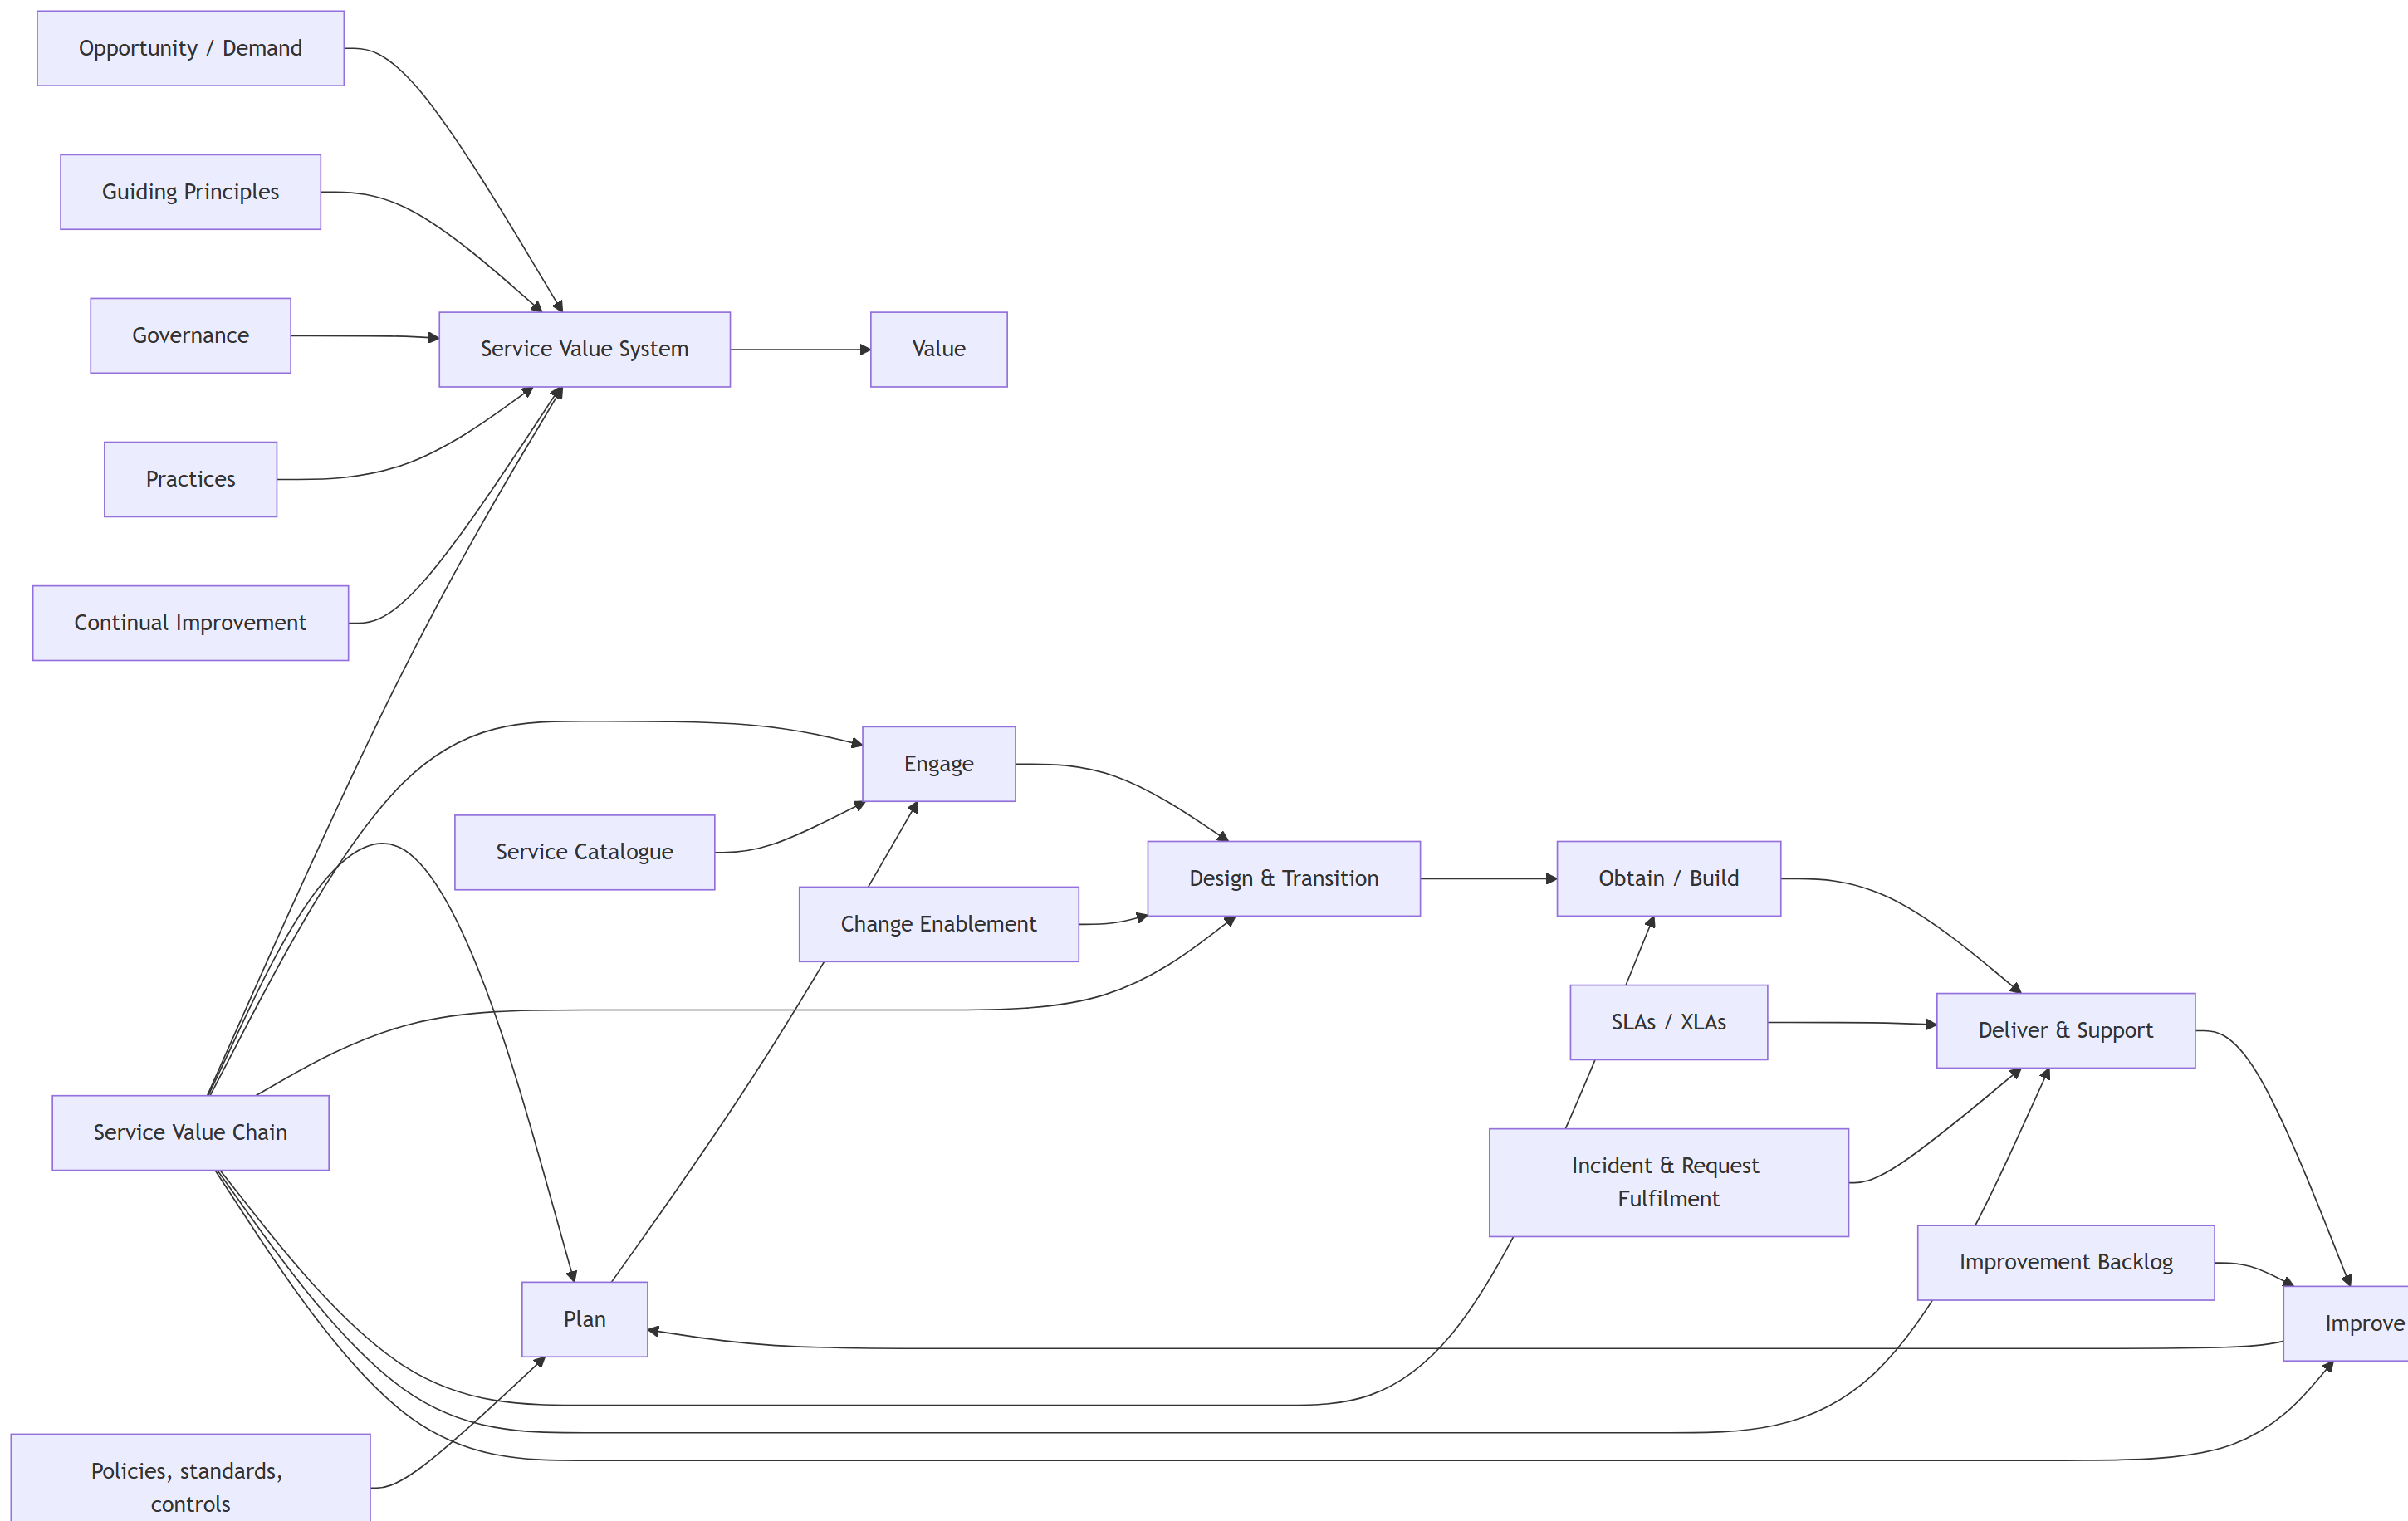
\includegraphics[width=18.53in,height=11.71in]{itil4_files/figure-latex/mermaid-figure-1.png}

The SVS describes how the organisation's components and activities work
together to enable value co-creation. It connects governance,
principles, practices, improvement, and operational activity into one
integrated model.

\begin{center}\rule{0.5\linewidth}{0.5pt}\end{center}

\section{History and Evolution}\label{history-and-evolution}

\begin{longtable}[]{@{}
  >{\raggedright\arraybackslash}p{(\linewidth - 4\tabcolsep) * \real{0.3333}}
  >{\raggedright\arraybackslash}p{(\linewidth - 4\tabcolsep) * \real{0.3333}}
  >{\raggedright\arraybackslash}p{(\linewidth - 4\tabcolsep) * \real{0.3333}}@{}}
\toprule\noalign{}
\begin{minipage}[b]{\linewidth}\raggedright
Version
\end{minipage} & \begin{minipage}[b]{\linewidth}\raggedright
Year
\end{minipage} & \begin{minipage}[b]{\linewidth}\raggedright
Key Changes
\end{minipage} \\
\midrule\noalign{}
\endhead
\bottomrule\noalign{}
\endlastfoot
ITIL v1 & 1989--1996 & Foundational library of IT service management
guidance \\
ITIL v2 & 2000--2001 & Consolidated guidance around service support and
service delivery \\
ITIL v3 & 2007 & Lifecycle model introduced: strategy, design,
transition, operation, CSI \\
ITIL 2011 Edition & 2011 & Refined lifecycle guidance and glossary,
clarified practices \\
ITIL 4 & 2019 & Introduced SVS, service value chain, four dimensions,
guiding principles, and 34 practices \\
ITIL Foundation (Version 5) / Bridge & 2025--2026 & New certification
evolution published by PeopleCert; ITIL 4 remains the core prior
framework and installed base \\
\end{longtable}

ITIL evolved from a process-heavy service support model into a broader
value and operating model for digital services. The major shift in ITIL
4 was the move from the older lifecycle structure to a more flexible
system that works better with Agile, DevOps, Lean, and product-based
delivery.

For this chapter, the focus remains on \textbf{ITIL 4} because it is the
framework most organisations currently reference when discussing the
service value system, 34 practices, and the modern IT service management
operating model.

\begin{center}\rule{0.5\linewidth}{0.5pt}\end{center}

\section{Core Principles}\label{core-principles}

ITIL 4 uses seven guiding principles that can be applied in nearly any
service management context:

\begin{enumerate}
\def\labelenumi{\arabic{enumi}.}
\item
  \textbf{Focus on value}\\
  Every activity should connect to value for customers, users, and the
  organisation.
\item
  \textbf{Start where you are}\\
  Assess current capabilities, services, tools, and relationships before
  redesigning or replacing them.
\item
  \textbf{Progress iteratively with feedback}\\
  Improve in manageable increments and learn continuously.
\item
  \textbf{Collaborate and promote visibility}\\
  Make work visible, reduce silos, and involve the right stakeholders.
\item
  \textbf{Think and work holistically}\\
  Manage services as systems, not isolated teams or processes.
\item
  \textbf{Keep it simple and practical}\\
  Use only the controls, steps, and documentation that genuinely add
  value.
\item
  \textbf{Optimise and automate}\\
  Standardise first where sensible, then automate repetitive and
  scalable work.
\end{enumerate}

These principles are especially valuable because ITIL 4 is designed to
be adaptable. The framework gives structure, but these principles help
leaders make balanced decisions without becoming overly bureaucratic.

\begin{center}\rule{0.5\linewidth}{0.5pt}\end{center}

\section{Governance Structure}\label{governance-structure}

\subsection{Governance, Service Management, and
Operations}\label{governance-service-management-and-operations}

ITIL 4 includes governance as a formal part of the Service Value System.
This is important because service management is not only an operational
discipline; it also requires policy direction, prioritisation, risk
oversight, and performance review.

A practical governance structure for ITIL 4 often includes:

\begin{itemize}
\tightlist
\item
  a board or executive forum providing strategic direction;
\item
  a CIO or service executive accountable for service performance and
  value;
\item
  service owners accountable for individual end-to-end services;
\item
  practice owners accountable for the design and performance of
  practices such as incident, change enablement, or service level
  management;
\item
  operational teams responsible for execution; and
\item
  assurance, security, risk, and audit teams providing oversight and
  challenge.
\end{itemize}

\subsection{Service Value Chain
Activities}\label{service-value-chain-activities}

\begin{longtable}[]{@{}
  >{\raggedright\arraybackslash}p{(\linewidth - 2\tabcolsep) * \real{0.5000}}
  >{\raggedright\arraybackslash}p{(\linewidth - 2\tabcolsep) * \real{0.5000}}@{}}
\toprule\noalign{}
\begin{minipage}[b]{\linewidth}\raggedright
Activity
\end{minipage} & \begin{minipage}[b]{\linewidth}\raggedright
Description
\end{minipage} \\
\midrule\noalign{}
\endhead
\bottomrule\noalign{}
\endlastfoot
Plan & Shared understanding of vision, current state, improvement
priorities, and direction. \\
Improve & Continual improvement of products, services, practices, and
all value chain activities. \\
Engage & Understanding stakeholder needs, maintaining relationships, and
ensuring transparency. \\
Design \& Transition & Ensuring new or changed services meet stakeholder
expectations for quality, cost, and time to market. \\
Obtain / Build & Acquiring, developing, and implementing service
components. \\
Deliver \& Support & Operating services and supporting users according
to agreed expectations. \\
\end{longtable}

\subsection{Four Dimensions of Service
Management}\label{four-dimensions-of-service-management}

\begin{longtable}[]{@{}
  >{\raggedright\arraybackslash}p{(\linewidth - 2\tabcolsep) * \real{0.5000}}
  >{\raggedright\arraybackslash}p{(\linewidth - 2\tabcolsep) * \real{0.5000}}@{}}
\toprule\noalign{}
\begin{minipage}[b]{\linewidth}\raggedright
Dimension
\end{minipage} & \begin{minipage}[b]{\linewidth}\raggedright
Description
\end{minipage} \\
\midrule\noalign{}
\endhead
\bottomrule\noalign{}
\endlastfoot
Organisations and People & Roles, culture, structure, competencies, and
workforce capacity needed to deliver services. \\
Information and Technology & Data, knowledge, applications,
infrastructure, automation, and supporting tools. \\
Partners and Suppliers & External providers, contracts, sourcing models,
and ecosystem dependencies. \\
Value Streams and Processes & End-to-end workflows, controls,
activities, and measurement paths that produce outcomes. \\
\end{longtable}

The four dimensions help prevent service design from being too narrow. A
change that looks good from a tooling perspective may still fail because
of skills, supplier, process, or governance gaps.

\begin{center}\rule{0.5\linewidth}{0.5pt}\end{center}

\section{Practices}\label{practices}

ITIL 4 defines \textbf{34 management practices}, grouped into three
families.

\subsection{General Management
Practices}\label{general-management-practices}

\begin{longtable}[]{@{}
  >{\raggedright\arraybackslash}p{(\linewidth - 2\tabcolsep) * \real{0.5000}}
  >{\raggedright\arraybackslash}p{(\linewidth - 2\tabcolsep) * \real{0.5000}}@{}}
\toprule\noalign{}
\begin{minipage}[b]{\linewidth}\raggedright
Practice
\end{minipage} & \begin{minipage}[b]{\linewidth}\raggedright
Purpose
\end{minipage} \\
\midrule\noalign{}
\endhead
\bottomrule\noalign{}
\endlastfoot
Architecture Management & Align technology and services with
organisational strategy and target-state design. \\
Continual Improvement & Improve products, services, and practices on an
ongoing basis. \\
Information Security Management & Protect information needed by the
organisation. \\
Knowledge Management & Ensure knowledge is captured, shared, and used
effectively. \\
Measurement and Reporting & Support good decisions through meaningful
information and reporting. \\
Organisational Change Management & Prepare people and organisations for
change. \\
Portfolio Management & Ensure the right mix of investments, services,
and initiatives. \\
Project Management & Plan and control temporary change initiatives. \\
Relationship Management & Build and sustain stakeholder
relationships. \\
Risk Management & Identify, assess, and treat uncertainty. \\
Financial Management for Services & Plan, allocate, and control
service-related costs and value. \\
Strategy Management & Define direction, priorities, and positioning. \\
Supplier Management & Manage supplier relationships and performance. \\
Workforce and Talent Management & Build the capacity and capabilities
needed for service delivery. \\
\end{longtable}

\subsection{Service Management
Practices}\label{service-management-practices}

\begin{longtable}[]{@{}
  >{\raggedright\arraybackslash}p{(\linewidth - 2\tabcolsep) * \real{0.5000}}
  >{\raggedright\arraybackslash}p{(\linewidth - 2\tabcolsep) * \real{0.5000}}@{}}
\toprule\noalign{}
\begin{minipage}[b]{\linewidth}\raggedright
Practice
\end{minipage} & \begin{minipage}[b]{\linewidth}\raggedright
Purpose
\end{minipage} \\
\midrule\noalign{}
\endhead
\bottomrule\noalign{}
\endlastfoot
Availability Management & Ensure services meet agreed availability
targets. \\
Business Analysis & Translate stakeholder needs into requirements and
improvement opportunities. \\
Capacity and Performance Management & Ensure services and resources
perform to current and future needs. \\
Change Enablement & Maximise successful changes while controlling
risk. \\
Incident Management & Restore normal service as quickly as possible
after disruption. \\
IT Asset Management & Manage lifecycle, control, and value of IT
assets. \\
Monitoring and Event Management & Observe services, components, and
events to support stability and response. \\
Problem Management & Reduce the likelihood and impact of incidents by
managing root causes and workarounds. \\
Release Management & Make new and changed services or features available
for use. \\
Service Catalogue Management & Provide accurate information about
available services and offers. \\
Service Configuration Management & Maintain trusted information about
configuration items and their relationships. \\
Service Continuity Management & Ensure the organisation can continue or
recover services after disruption. \\
Service Design & Design products and services fit for purpose and
use. \\
Service Desk & Provide the primary point of contact for users and many
operational workflows. \\
Service Level Management & Set, monitor, and improve service targets and
service experience. \\
Service Request Management & Fulfil pre-defined user requests
efficiently and consistently. \\
Service Validation and Testing & Confirm that services meet design and
business requirements. \\
\end{longtable}

\subsection{Technical Management
Practices}\label{technical-management-practices}

\begin{longtable}[]{@{}
  >{\raggedright\arraybackslash}p{(\linewidth - 2\tabcolsep) * \real{0.5000}}
  >{\raggedright\arraybackslash}p{(\linewidth - 2\tabcolsep) * \real{0.5000}}@{}}
\toprule\noalign{}
\begin{minipage}[b]{\linewidth}\raggedright
Practice
\end{minipage} & \begin{minipage}[b]{\linewidth}\raggedright
Purpose
\end{minipage} \\
\midrule\noalign{}
\endhead
\bottomrule\noalign{}
\endlastfoot
Deployment Management & Move new or changed components into live or test
environments. \\
Infrastructure and Platform Management & Oversee infrastructure and
platform components supporting services. \\
Software Development and Management & Develop, maintain, and control
software throughout its lifecycle. \\
\end{longtable}

In practice, organisations rarely implement all practices at the same
level of maturity from the start. A phased adoption approach often
begins with service desk, incident, request, change enablement, problem,
service level, monitoring, and configuration-related capabilities, then
expands into broader governance, portfolio, supplier, and improvement
disciplines.

\begin{center}\rule{0.5\linewidth}{0.5pt}\end{center}

\section{Documentation and Artefacts}\label{documentation-and-artefacts}

This section defines the key documents produced within the framework and
the roles responsible for creating, approving, and maintaining them.

\subsection{ITIL 4 Documentation RACI
Matrix}\label{itil-4-documentation-raci-matrix}

\textbf{Legend:} R = Responsible, A = Accountable, C = Consulted, I =
Informed

\begin{longtable}[]{@{}
  >{\raggedright\arraybackslash}p{(\linewidth - 18\tabcolsep) * \real{0.0769}}
  >{\raggedleft\arraybackslash}p{(\linewidth - 18\tabcolsep) * \real{0.1026}}
  >{\raggedleft\arraybackslash}p{(\linewidth - 18\tabcolsep) * \real{0.1026}}
  >{\raggedleft\arraybackslash}p{(\linewidth - 18\tabcolsep) * \real{0.1026}}
  >{\raggedleft\arraybackslash}p{(\linewidth - 18\tabcolsep) * \real{0.1026}}
  >{\raggedleft\arraybackslash}p{(\linewidth - 18\tabcolsep) * \real{0.1026}}
  >{\raggedleft\arraybackslash}p{(\linewidth - 18\tabcolsep) * \real{0.1026}}
  >{\raggedleft\arraybackslash}p{(\linewidth - 18\tabcolsep) * \real{0.1026}}
  >{\raggedleft\arraybackslash}p{(\linewidth - 18\tabcolsep) * \real{0.1026}}
  >{\raggedleft\arraybackslash}p{(\linewidth - 18\tabcolsep) * \real{0.1026}}@{}}
\toprule\noalign{}
\begin{minipage}[b]{\linewidth}\raggedright
Document / Artefact
\end{minipage} & \begin{minipage}[b]{\linewidth}\raggedleft
Executive Sponsor / CIO
\end{minipage} & \begin{minipage}[b]{\linewidth}\raggedleft
Head of ITSM / SMO
\end{minipage} & \begin{minipage}[b]{\linewidth}\raggedleft
Service Owner
\end{minipage} & \begin{minipage}[b]{\linewidth}\raggedleft
Practice Owner
\end{minipage} & \begin{minipage}[b]{\linewidth}\raggedleft
Service Desk / Operations Manager
\end{minipage} & \begin{minipage}[b]{\linewidth}\raggedleft
Enterprise Architect
\end{minipage} & \begin{minipage}[b]{\linewidth}\raggedleft
Risk / Security / Compliance
\end{minipage} & \begin{minipage}[b]{\linewidth}\raggedleft
Supplier Manager
\end{minipage} & \begin{minipage}[b]{\linewidth}\raggedleft
Internal Audit
\end{minipage} \\
\midrule\noalign{}
\endhead
\bottomrule\noalign{}
\endlastfoot
Service Management Policy & A & R & C & C & I & C & C & I & I \\
Service Management Operating Model & A & R & C & C & C & C & C & I &
I \\
Service Portfolio & A & R & C & I & I & C & I & I & I \\
Service Catalogue & I & A & R & C & C & I & I & I & I \\
Service Definition / Service Design Package & I & C & A/R & C & C & C &
C & I & I \\
Service Level Policy & I & A & R & C & C & I & C & I & I \\
SLA / OLA / Underpinning Contract & I & C & A/R & C & C & I & C & C &
I \\
Service Review Report & I & A & R & C & C & I & C & I & I \\
Service Improvement Register & I & A & R & C & C & I & C & I & I \\
Continual Improvement Plan & I & A & R & C & C & I & C & I & I \\
Incident Management Policy & I & A & C & R & C & I & C & I & I \\
Major Incident Procedure & I & A & C & R & R & I & C & I & I \\
Incident Record / Major Incident Record & I & I & C & C & A/R & I & I &
I & I \\
Problem Management Policy & I & A & C & R & C & I & C & I & I \\
Problem Record / Known Error Record & I & I & C & A & R & I & I & I &
I \\
Change Enablement Policy & I & A & C & R & C & I & C & I & I \\
Change Record / Change Schedule & I & I & C & A & R & I & C & I & I \\
CAB Terms of Reference & I & A & C & R & C & I & C & I & I \\
Release and Deployment Plan & I & C & A & C & R & C & C & I & I \\
Configuration Management Policy & I & A & C & R & C & C & C & I & I \\
CMDB / Service Configuration Model & I & I & C & A & R & C & I & I &
I \\
Availability and Capacity Plan & I & C & A/R & C & C & C & I & I & I \\
Monitoring and Event Model & I & C & C & A & R & C & C & I & I \\
Service Continuity Plan / DR Plan & I & C & A & C & R & C & C & I & C \\
Knowledge Management Policy & I & A & C & R & C & I & I & I & I \\
Knowledge Articles / Runbooks & I & I & C & C & A/R & I & I & I & I \\
Supplier Management Policy & I & A & C & I & I & I & C & R & I \\
Supplier Performance Report & I & C & C & I & I & I & C & A/R & I \\
Information Security Policy Interface & I & C & C & I & C & I & A/R & I
& C \\
Audit and Compliance Evidence Pack & I & C & C & C & C & I & R & I &
A/C \\
KPI / Service Performance Dashboard & I & A & R & C & C & I & C & I &
I \\
Lessons Learned Repository & I & A & C & C & R & I & C & I & I \\
\end{longtable}

The exact role design varies by organisation, but the key pattern is
stable: service owners are accountable for end-to-end service outcomes,
practice owners are accountable for the health of specific practices,
and operational teams are responsible for day-to-day execution and
evidence generation.

\begin{center}\rule{0.5\linewidth}{0.5pt}\end{center}

\section{Integration with Other
Frameworks}\label{integration-with-other-frameworks}

\begin{longtable}[]{@{}
  >{\raggedright\arraybackslash}p{(\linewidth - 2\tabcolsep) * \real{0.5000}}
  >{\raggedright\arraybackslash}p{(\linewidth - 2\tabcolsep) * \real{0.5000}}@{}}
\toprule\noalign{}
\begin{minipage}[b]{\linewidth}\raggedright
Framework
\end{minipage} & \begin{minipage}[b]{\linewidth}\raggedright
Relationship
\end{minipage} \\
\midrule\noalign{}
\endhead
\bottomrule\noalign{}
\endlastfoot
COBIT & Provides enterprise governance, control objectives, and
assurance structure above ITIL service management. \\
TOGAF & Provides target-state architecture, standards, and design
governance that shape services and platforms. \\
PRINCE2 & Governs projects that introduce or change services,
environments, and supporting capabilities. \\
MSP & Coordinates transformation programmes that change multiple
services and operating models together. \\
DevOps / Agile & Complements ITIL 4 by accelerating flow, feedback,
automation, and cross-functional delivery. \\
ISO/IEC 20000 & Offers a certifiable service management standard aligned
with many ITIL practices. \\
ISO 27001 / NIS2 / DORA & Add security, resilience, compliance, and
operational control requirements around services. \\
\end{longtable}

ITIL 4 works particularly well as the operational layer in a broader
governance stack:

\begin{itemize}
\tightlist
\item
  \textbf{COBIT} defines governance and control expectations;
\item
  \textbf{TOGAF} defines architecture direction and standards;
\item
  \textbf{ITIL 4} defines service management and operational value
  delivery;
\item
  \textbf{PRINCE2 / MSP} drive controlled change and transformation.
\end{itemize}

\begin{center}\rule{0.5\linewidth}{0.5pt}\end{center}

\section{Implementation Approach}\label{implementation-approach}

A pragmatic ITIL 4 adoption normally works best in phases rather than as
a large one-off redesign.

\begin{enumerate}
\def\labelenumi{\arabic{enumi}.}
\item
  \textbf{Assess the current state}\\
  Review services, support model, tooling, pain points, service levels,
  maturity, and stakeholder expectations.
\item
  \textbf{Define the target operating model}\\
  Clarify service ownership, governance forums, practice ownership,
  metrics, value streams, and integration with architecture, security,
  and delivery.
\item
  \textbf{Prioritise core practices}\\
  Start with the most business-critical areas such as service desk,
  incident, request, change enablement, problem, service level,
  monitoring, and knowledge.
\item
  \textbf{Design workflows and controls}\\
  Simplify handoffs, clarify escalation paths, define policies, and
  remove unnecessary bureaucracy.
\item
  \textbf{Enable tooling and data}\\
  Implement service management tooling, knowledge structures,
  CMDB/service configuration data where justified, dashboards, and
  automation.
\item
  \textbf{Establish measurement and review}\\
  Use service reviews, practice reviews, trend reporting, and continual
  improvement backlogs.
\item
  \textbf{Scale and integrate}\\
  Extend the model into supplier governance, continuity, portfolio
  alignment, product teams, cloud operations, and enterprise governance.
\end{enumerate}

A successful ITIL 4 implementation is usually less about copying every
practice verbatim and more about building a coherent, measurable service
operating model that fits the organisation.

\begin{center}\rule{0.5\linewidth}{0.5pt}\end{center}

\section{KPIs and Metrics}\label{kpis-and-metrics}

\begin{longtable}[]{@{}
  >{\raggedright\arraybackslash}p{(\linewidth - 2\tabcolsep) * \real{0.5000}}
  >{\raggedright\arraybackslash}p{(\linewidth - 2\tabcolsep) * \real{0.5000}}@{}}
\toprule\noalign{}
\begin{minipage}[b]{\linewidth}\raggedright
KPI
\end{minipage} & \begin{minipage}[b]{\linewidth}\raggedright
Measurement
\end{minipage} \\
\midrule\noalign{}
\endhead
\bottomrule\noalign{}
\endlastfoot
Service Availability & \% service uptime against agreed target \\
Mean Time to Restore Service (MTRS) & Average elapsed time to restore
normal service \\
First Contact Resolution & \% incidents or requests resolved at first
contact \\
Incident Volume Trend & Number of incidents by service, severity, or
period \\
Major Incident Frequency & Number of priority incidents over time \\
Change Success Rate & \% changes implemented without incident, rollback,
or significant disruption \\
Emergency Change Ratio & \% changes raised as emergency changes \\
Problem Backlog Age & Average age of open problem records \\
Reopened Incident Rate & \% incidents reopened after apparent
resolution \\
Request Fulfilment Time & Average time to complete standard requests \\
SLA Achievement & \% targets achieved per service or customer group \\
Customer Satisfaction / Experience & CSAT, CES, or XLA-linked
measures \\
Knowledge Article Reuse & Number or \% of tickets resolved using
knowledge content \\
Supplier Performance & \% contractual targets met by supplier \\
Improvement Delivery Rate & \% improvement actions completed on time \\
\end{longtable}

Metrics should be balanced. If an organisation only measures speed,
teams may close tickets too early. If it only measures compliance, teams
may become slow and overly procedural. ITIL 4 works best when service
performance, experience, risk, and improvement are measured together.

\begin{center}\rule{0.5\linewidth}{0.5pt}\end{center}

\section{Benefits}\label{benefits}

\begin{itemize}
\tightlist
\item
  Stronger alignment between services and business value
\item
  Clearer service ownership and accountability
\item
  Better incident, change, problem, and request control
\item
  Improved user experience and service transparency
\item
  Better integration across operations, architecture, suppliers, and
  delivery
\item
  More structured continual improvement
\item
  Stronger auditability and evidence for operational governance
\item
  A framework that can coexist with Agile, DevOps, and product operating
  models
\end{itemize}

\begin{center}\rule{0.5\linewidth}{0.5pt}\end{center}

\section{Limitations}\label{limitations}

\begin{itemize}
\tightlist
\item
  Can become bureaucratic if implemented as rigid process overhead
\item
  Requires disciplined role ownership and governance to work well
\item
  Tooling can dominate thinking if the operating model is weak
\item
  Some organisations over-focus on ticketing rather than service value
\item
  CMDB and configuration efforts can become expensive if over-engineered
\item
  Benefits depend heavily on cultural adoption, not just documented
  process
\end{itemize}

\begin{center}\rule{0.5\linewidth}{0.5pt}\end{center}

\section{Practical Use Case}\label{practical-use-case}

\subsection{Example: Stabilising Service Operations After Cloud
Transformation}\label{example-stabilising-service-operations-after-cloud-transformation}

An organisation has completed a rapid cloud migration but now faces
frequent incidents, unclear ownership, inconsistent changes, weak
supplier coordination, and poor visibility of service performance.

A practical ITIL 4 response would include:

\begin{itemize}
\tightlist
\item
  defining the critical business services and assigning service owners;
\item
  establishing service catalogue entries and service level targets;
\item
  strengthening incident, major incident, request, problem, and change
  enablement practices;
\item
  creating runbooks, knowledge articles, and event monitoring models;
\item
  clarifying relationships between internal platform teams and cloud
  suppliers;
\item
  setting up service review forums and improvement backlogs; and
\item
  measuring restoration time, change success, major incident frequency,
  and customer satisfaction.
\end{itemize}

The result is not simply better support. It is a more controlled service
operating model in which cloud platforms, suppliers, operations teams,
and business stakeholders work through shared governance, shared service
definitions, and measurable value outcomes.

\begin{center}\rule{0.5\linewidth}{0.5pt}\end{center}

\section{Closing View}\label{closing-view}

ITIL 4 is most powerful when used as a practical operating model for
service value co-creation rather than a strict compliance checklist. In
an enterprise governance landscape, it provides the link between
strategy, architecture, change, and daily service delivery.

For your wider governance book, ITIL 4 sits naturally after
\textbf{COBIT} and \textbf{TOGAF}:

\begin{itemize}
\tightlist
\item
  \textbf{COBIT} explains how enterprise I\&T should be governed;
\item
  \textbf{TOGAF} explains how target-state architecture should be
  designed and governed; and
\item
  \textbf{ITIL 4} explains how services should be designed, operated,
  supported, and improved to realise value in practice.
\end{itemize}

\section{References}\label{references}

\begin{itemize}
\tightlist
\item
  AXELOS. \emph{ITIL 4 Foundation}. AXELOS.
\item
  AXELOS. \emph{Reader's Manual: ITIL 4 Practice Guide}. AXELOS.
\item
  AXELOS. \emph{Architecture Management: ITIL 4 Practice Guide}. AXELOS.
\item
  AXELOS. \emph{Measurement and Reporting Management: ITIL 4 Practice
  Guide}. AXELOS.
\item
  PeopleCert. \emph{ITIL 4 Practice Guides -- a Hidden Gem}. PeopleCert.
\item
  PeopleCert. \emph{ITIL 4 Practice Guides Masterclass Series}.
  PeopleCert.
\item
  PeopleCert. \emph{ITIL Framework / ITIL 4 Foundation}. PeopleCert.
\item
  PeopleCert. \emph{PeopleCert Library}. PeopleCert.
\item
  PeopleCert. \emph{What's Changing in ITIL?} PeopleCert FAQ.
\end{itemize}




\end{document}
